Zum Schluss werden die gemessenen Ergebnisse aller Szenarien noch einmal gesammelt zusammengefasst. Dabei werden auch die Ergebnisse von Szenario 5 mit den Seeds 3 und 10 eingeschlossen. Tabelle~\ref{tab:zusammen} listet alle gemessenen Durchschnittswerte auf.
\begin{table}[!htbp]
	\centering\small
	\begin{tblr}{
		colspec={lcrrrrr},
		row{1} = {c,font=\bfseries},
		}
		\toprule
		Szenario & System & \ac{fps} & {\ac{cpu}\\ (\si{\percent})} & {\ac{gpu}\\ (\si{\percent})} & {\ac{ram}\\ (\si{\mega\byte})} & { \ac{ram} kurz \\ (\si{\mega\byte\per\second})}\\
		\midrule
		\SetCell[r=3]{} 1 Hexagon				
			& SystemA & 337& 13& 36& 576&  70\\
			& SystemB &1133& 18& 38& 947& 274\\
			& $\Delta$ &$+\SI{226}{\percent}$& $+\SI{38}{\percent}$& $+\SI{5}{\percent}$& $+\SI{64}{\percent}$& $+\SI{291}{\percent}$\\
		\midrule
		\SetCell[r=3]{}2 Halb-Würfel			
			& SystemA & 253& 13& 60& 643&  53\\
			& SystemB & 417& 18& 94& 941& 101\\
			& $\Delta$ &$+\SI{65}{\percent}$& $+\SI{38}{\percent}$& $+\SI{57}{\percent}$& $+\SI{46}{\percent}$& $+\SI{91}{\percent}$\\
		\midrule
		\SetCell[r=3]{}3 Welt-Statisch		
			& SystemA & 201& 13& 40&1243&  94\\
			& SystemB & 468& 23& 71&1793& 208\\
			& $\Delta$ &$+\SI{133}{\percent}$& $+\SI{77}{\percent}$& $+\SI{78}{\percent}$& $+\SI{44}{\percent}$& $+\SI{121}{\percent}$\\
		\midrule
		\SetCell[r=3]{}4 Welt-Rotation		
			& SystemA & 134& 13& 37& 1267&101\\
			& SystemB & 378& 23& 53& 1441&187\\
			& $\Delta$ &$+\SI{182}{\percent}$& $+\SI{77}{\percent}$& $+\SI{43}{\percent}$& $+\SI{14}{\percent}$& $+\SI{85}{\percent}$\\
		\midrule
		\SetCell[r=3]{}5 Welt-Gehen (0)	
			& SystemA & 128& 27& 34& 1215&114\\
			& SystemB & 381& 36& 42& 1881&248\\
			& $\Delta$ &$+\SI{198}{\percent}$& $+\SI{33}{\percent}$& $+\SI{24}{\percent}$& $+\SI{55}{\percent}$& $+\SI{118}{\percent}$\\
		\midrule
		\SetCell[r=3]{}5 Welt-Gehen (3)	
			& SystemA &  72& 34& 28& 1194&85\\
			& SystemB & 190& 42& 34& 1424&198\\
			& $\Delta$ &$+\SI{164}{\percent}$& $+\SI{24}{\percent}$& $+\SI{21}{\percent}$& $+\SI{19}{\percent}$& $+\SI{133}{\percent}$\\
		\midrule
		\SetCell[r=3]{}5 Welt-Gehen (10)	
			& SystemA & 148& 25& 32& 1125&146\\
			& SystemB & 481& 37& 35& 1505&281\\
			& $\Delta$ &$+\SI{225}{\percent}$& $+\SI{48}{\percent}$& $+\SI{9}{\percent}$& $+\SI{34}{\percent}$& $+\SI{92}{\percent}$\\
		\midrule
		\midrule
		\SetCell[r=3]{}Gesamtdurchschnitt 
			& SystemA & 182& 20& 38& 1038&95\\
			& SystemB & 493& 28& 52& 1418&214\\
			& $\Delta$ &$+\SI{170}{\percent}$& $+\SI{40}{\percent}$& $+\SI{37}{\percent}$& $+\SI{37}{\percent}$& $+\SI{115}{\percent}$\\
			\bottomrule
	\end{tblr}
	\caption{Durchschnittliche Messwerte in den allen Szenarien der Performanceanalyse.}\label{tab:zusammen}
\end{table}
Die Zeilen, die durch $\Delta$ gekennzeichnet sind, enthalten die relative Veränderung von SystemB im Vergleich zu SystemA. Betrachtet man diese Veränderung, ist zu erkennen, dass die Werte von SystemB ausnahmslos in allen Messbereichen gestiegen sind. Das schließt die Framerate aber auch den Speicherverbrauch ein. Der größte relative und absolute Zuwachs in der Bildwiederholrate ist in Szenario 1: Hexagon zu beobachten. In allen Szenarien ist der Zuwachs größer als \SI{100}{\fps}. Leider ist aus den Messungen nicht zu erkennen, welcher Teil der gestiegenen Auslastung von \ac{cpu} und \ac{gpu} aus der besseren Nutzung durch Multithreading hervorgeht und welchen Anteil der für die Implementierung notwendige Overhead beispielsweise durch die Zwischenspeicherung der Renderables ausmacht. Die stark gestiegene Framerate stellt allerdings sicher, dass ohne Zweifel eine bessere Nutzung der zur Verfügung stehenden Leistung durch die neue nebenläufige Architektur von SystemB ermöglicht wird.

Die Betrachtung der Messungen von Szenario 5: Welt-Gehen mit unterschiedlichen Seeds zeigt, dass diese einen erheblichen Einfluss auf die Framerate haben. Das lässt sich leicht durch die Anzahl der zu zeichnenden Objekte erklären. In Seed 3 ist die Startposition der Kamera unterirdisch in einer Berglandschaft. Dadurch enthält beinahe das gesamte Sichtfeld Chunks, die verarbeitet werden müssen. Das sorgt für eine besonders hohe Auslastung der \ac{cpu}, die all diese Chunks verarbeiten muss. Hier zeigt sich auch, dass weiterhin die \ac{cpu} in diesem Testsystem den Flaschenhals für die Leistung darstellt. Die \ac{gpu} hat in diesem Szenario mit dem Seed 3 die niedrigste Auslastung über alle Szenarien hinweg.

Durchschnittlich kann eine Gesamtsteigerung von \SI{170}{\percent} in der Framerate beobachtet werden, in absoluten Werten ist das eine Steigerung von \SI{311}{\fps}.

Weiterhin wird mit einem Plus von \SI{115}{\percent} etwa doppelt soviel Speicher für die kurzfristige Erzeugung von Objekten genutzt. Da die Erzeugung von Objekten relativ zeitaufwändig ist, kann hier in Zukunft unter geschickter Nutzung von Objekt-Chaches eine weitere Leistungssteigerung erreicht werden. Es ist zu beachten, dass mit einer höheren Framerate die Codestellen, in denen Objekte erzeugt werden, häufiger aufgerufen werden. Daher lässt sich bei gestiegener Bildwiederholrate auch ein gestiegener Speicherverbrauch erwarten. In den Messungen lässt sich hierfür allerdings keine Korrelation erkennen, wie Abbildung~\ref{fig:Scatterplot} zeigt. In der Abbildung sind ist der durchschnittliche Zuwachs der \ac{fps} gegen den durchschnittlichen Zuwachs des Speicherverbrauchs für die Erzeugung kurzfristig genutzter Objekte (\ac{ram} kurz) aufgetragen. 
\begin{figure}
	\centering
	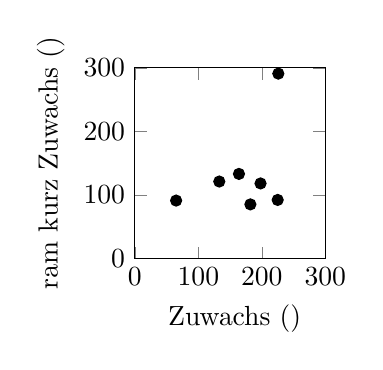
\begin{tikzpicture}
		\begin{axis}[
			no markers=false,
			ymin=0,
			xmin=0,
			xmax=300,
			ymax=300,
			width=4cm,
			height=4cm,
			xlabel={\si{\fps} Zuwachs (\si{\percent})},
			ylabel={\ac{ram} kurz Zuwachs (\si{\percent})},
		]
		\addplot[
			only marks
	] table {
		fps ram
		226 291
		65 91
		133 121
		182 85
		198 118
		164 133
		225 92
		};
		\end{axis}
		\end{tikzpicture}
		\caption[Scatterplot der Durchschnittswerte für \glsentryshort{fps}- und kurzfristigen \glsentryshort{ram}-Nutzungs-Zuwachs.]{Scatterplot der Durchschnittswerte für \si{\fps}- und kurzfristigen \ac{ram}-Nutzungs-Zuwachs. Die Werte lassen keine Korrelation erkennen.}\label{fig:Scatterplot}
\end{figure}

Es ist nicht verwunderlich, dass der Gesamtspeicherverbrauch in der Blocklib von SystemA zu SystemB gestiegen ist, da beispielsweise für die Zwischenspeicherung der Renderables viele Daten doppelt gespeichert werden. 